\documentclass[12pt,a4paper]{article}
\usepackage[utf8]{inputenc}
\usepackage{amsmath}
\usepackage{amsfonts}
\usepackage{amssymb}
\usepackage{graphicx}
\usepackage{listings}
\begin{document}
\graphicspath{ {./images/} }
\DeclareGraphicsExtensions{.pdf,.png,.jpg}
\lstset{language=bash}      
\author{Steven L. Speek}
\title{GNUAmsterdam Debian Wheezy Installatie}
\date{\today}
\maketitle
\abstract{Nederlandse handleiding voor een Debian desktop installatie.}
\section{Algemene aanwijzingen}
\emph{Zeer belangrijk:} Iedere vraag die door het installatie programma aan jou wordt gesteld en waarover hieronder niets staat vermeldt beantwoordt je met de enter-toets.

Als de debian installer naar een nieuw scherm gaat, begint er in deze handleiding een nieuwe paragraaf
\section{Floppy station onklaar maken}
Floppy stations zijn een erfenis uit het verleden. Schakel de floppy ondersteuning in de BIOS uit. En maak de kabels verbonden met het floppy-station los.
\section{CDROM ophalen}
Op www.debian.org/distrib/, kies je een klein installatie-image voor jouw architectuur (meestal amd64, soms nog i686).
Brandt dit op een CDROM, dit zullen wij de installatie CDROM noemen.
\section{Installatie basissysteem}
Boot van de installatie CDROM. Je komt dan in een menu.
Je accepteert de eerste optie \textbf{Install} met enter.
\begin{figure}[h]
\centering
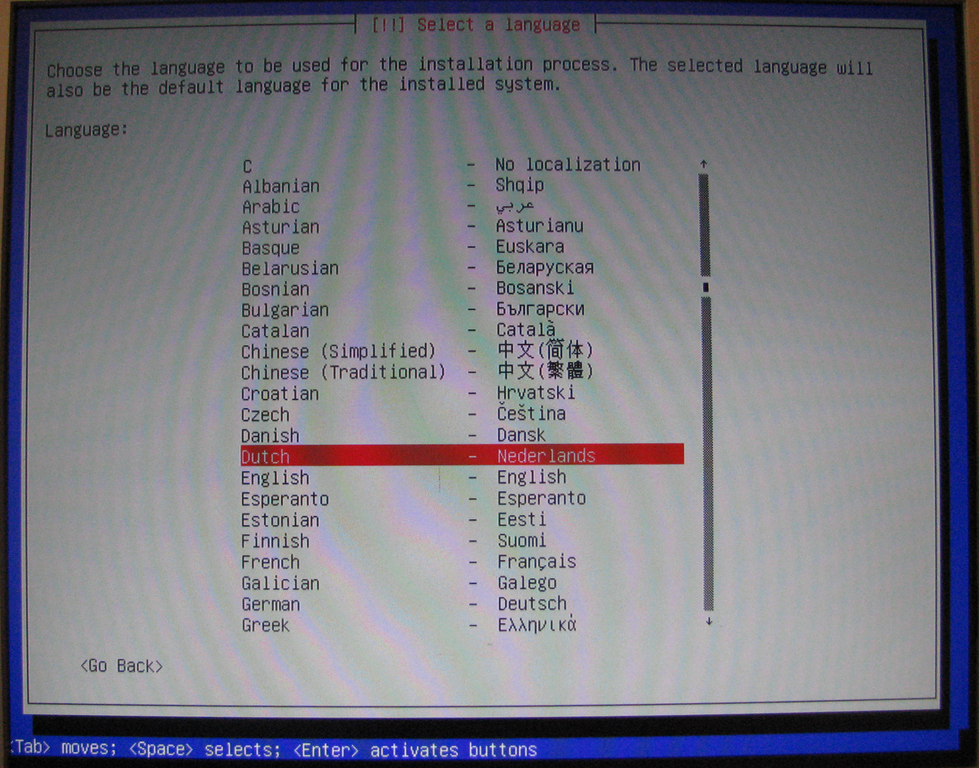
\includegraphics[width=0.8\textwidth]{taal-keuze-scherm}
\caption{Kies hier \textbf{Dutch} als taal.}
\label{fig:taal-keuze-scherm}
\end{figure}

Op het volgende scherm, zie figuur ~\ref{fig:taal-keuze-scherm},  kun je de taal kiezen; kies \textbf{Dutch} (pijltje omhoog en dan enter).


Regio/Land: \textbf{Nederland} en druk enter.

Voor de toetsenbordindeling kies je \textbf{American English}, druk op enter.

Na het laden van de aanvullende installatie modules. En vragen over ontbrekende firmware, die je allen met \textbf{nee} beantwoordt. Vul je \textbf{debian} in als computernaam en drukt op enter.
En vul je \textbf{lan} in bij domeinnaam en drukt op enter.

Nu moeten het root wachtwoord worden gezet.
Vul als root wachtwoord in \textbf{root} (bevestigen met enter), en doe dit nogmaals ter controle.

Je vult \textbf{Tux} in als volledige naam van de nieuwe aardse gebruiker.
De debian installer suggereert dan \textbf{tux} als gebruikersnaam.
Dat accepteer je met enter.

Als wachtwoord vul je \textbf{tux} in. Dit moet nog een keer worden bevestigd.
\section{Schijfindeling voor de verkoop}
Bij de schijfindeling kies je \textbf{Benut gehele schijf met LVM en encryptie}.

Nu moet je kiezen hoe de schijf gaat worden ingedeeld; je kiest de onderste optie \textbf{Afzondelijke /home, /usr, /var en /tmp partitie}.

Nadat je dit bevestigd hebt, gaat de installer de gehele disk wissen, dat kan even duren (in de orde van uren). Je mag dit annuleren.

Daarna wordt er om een wachtwoordzin gevraagd, je vult \textbf{gnu} in. Dit moet je nogmaals te controle doen.

Je moet nu bevestigen dat dit een zwakke wachtwoordzin is. 

Het partitie schema wordt nog eenmaal aan je getoond opdat je het nog een keer kunt controleren. Je bevestigt de voorgestelde keuze.

\begin{lstlisting}[language=bash]
$lsof -i :80
\end{lstlisting}
Shows open files.
\end{document}
